\documentclass{article}

\usepackage{graphicx} % Required for inserting images
\usepackage[T1]{fontenc} % Fuentas en español
\usepackage[spanish]{babel} % Traduccion a español del Lattex
\usepackage[skip=9pt plus2pt]{parskip} % Espaciado más ámplio
\usepackage{fancyhdr} % Footer y Header
\usepackage{fancyhdr}

% \fancyhead[locations]{content}
\fancyhead[L]{\item}
\fancyfoot[R]{Sergiy Khudoley}
\fancyfoot[L]{Sistemas Operativos - UBU}

\title{Sistemas Operativos - Práctica de Control II}
\author{Sergiy Khudoley}
\date{\today}

\begin{document}
\pagestyle{fancy}

\maketitle
\tableofcontents

% \newpage


\section{Preludio}
    Estoy iniciando este proyecto con conocimientos muy básicos del lenguaje de scripting \textbf{bash}. Los antecedentes que he podido tener de este lenguaje son más bien anecdóticos.

    Con esta práctica estoy teniendo mi primer contacto con un script relativamente complejo, y se puede observar en la \textbf{inconsistencia del formato} que utilizo para escribir el código. Este ha ido variando bastante desde mis primeros intentos hasta el momento presente.
    
    Apenas estoy aprendiendo la sintaxis básica y las posibles opciones de las que dispongo para atajar diferentes problemas. Viendo las \textbf{similitudes} y \textbf{diferencias} respecto a otros lenguajes de programación.

    Para mis primeros contactos  he utilizado de forma exhaustiva \textbf{ChatGPT}. Este me ha permitido ganar tracción con el lenguaje de forma extremadamente rápida. Pero pronto he encontrado que tenía un serio problema. Esto me producía \textbf{mucha inconsistencia} en el código.
    
    Al no conocer todavía las opciones disponibles, no sabía cual era la forma \textbf{óptima} o al menos que estilo me venía mejor en ese momento. Por ello, una vez me sentía más cómodo me empezó a ser más útil referirmente a soluciones encontradas en \textbf{Stackoverflow}.

    Por último, en la mayor parte del tiempo, simplemente me he referido al guión de la \textbf{práctica 6} dada en clase. Ya que habitualmente la mayor parte de dudas solían ser más bien dudas de sintaxis de resolución rápida.

    
    
\newpage
\section{Requerimientos}
    \subsection{Referencias}
        \subsubsection{Referenciar script original}
            Este script debe localizar todos los comentarios existentes de cualquier fichero \textbf{.sh} que se encuentre en un determinado directorio. Esto incluye posibles subdirectorios anidados.
    
            El script debe localizar todos estos ficheros y crear una numeración del tipo \textbf{\#ES\_10}, teniendo en cuenta que la referencia se genera con \textbf{dos letras} mayúsculas seguido de un \textbf{\_} y la numeración del comentario, comenzando el comentario por 10 e incrementandose de 10 en 10 posteriormente.
            
        \subsubsection{Creación de fichero para idiomas}
            El fichero de script generará otro grupo de ficheros, los que sean necesarios dependiendo de la cantidad de idiomas con los que esté trabajando con el prefijo de cada idioma y acabado en la extensión \textbf{.txt}.
        
        \subsubsection{Intercambio con comentarios externos}
            El script puede pedir seleccionar uno de los idiomas disponibles, y debe ser capaz de intercambiar los comentarios guardados en los fircheros \textbf{.txt} por sus respectivos comentarios numerados denre del fichero original.
        
        \subsubsection{Archivos de log}
            En caso de existitr algun problema en la sustitución de los comentarios, debe guardarse el comentario a insertar en un archivo \textbf{.log} para su posterior comprobación.
        
    \subsection{Idiomas}
        \subsubsection{Trabajando con multiples idiomas}
            El script genera un archivo oculto llamado \textbf{.idiomas} en el mismo directorio donde se guardarán los prefijos/idiomas a utilizar. Estos serán utilizados para pedir al usuario que idioma desea utilizar para el intercambio de comentarios y cuantos ficheros \textbf{.txt} debe generar al crear las referencias.
        \subsubsection{Agregando idiomas adicionales}
            El script permite también el insertado de nuevos idiomas para poder trabajar con ellos posteriormente.
\newpage
\section{Primera tentativa y proyecto de git}
    \subsection{Inicio del proyecto}
        Mi primer intento crear el script ha sido más bien erratico.
        
        He empezado a crear los procedimientos que necesitaba de forma procedural para ver que problemas me podría encontrar por el camino. Pronto me topé con el primer problema.Había decidido buscar los comentarios utilizando \textbf{grep}.
        
        Empezé buscando diferentes casos que escapaban al alcance del patrón que estaba utilizando. Esto hizo que le dedicara bastante esfuerzo sin realizar ningún avance significativo.
    
        A la vez el código empezó pronto a crecer más de lo que esperaba y a tener la necesidad de modificarlo. Tenía que empezar a plantearme el como estructurarlo.
    
        Aquí decidí empezar a dividir el código en funciones y plantearme como quería organizarlo.
    
        En este momento me sentía con fuerzas para realizar un planteamiento diferente. Ya no estaba tan centrado en el \textbf{como} sino en el \textbf{qué}. Este fue el punto de inflexión.

        \begin{figure}
            \centering
            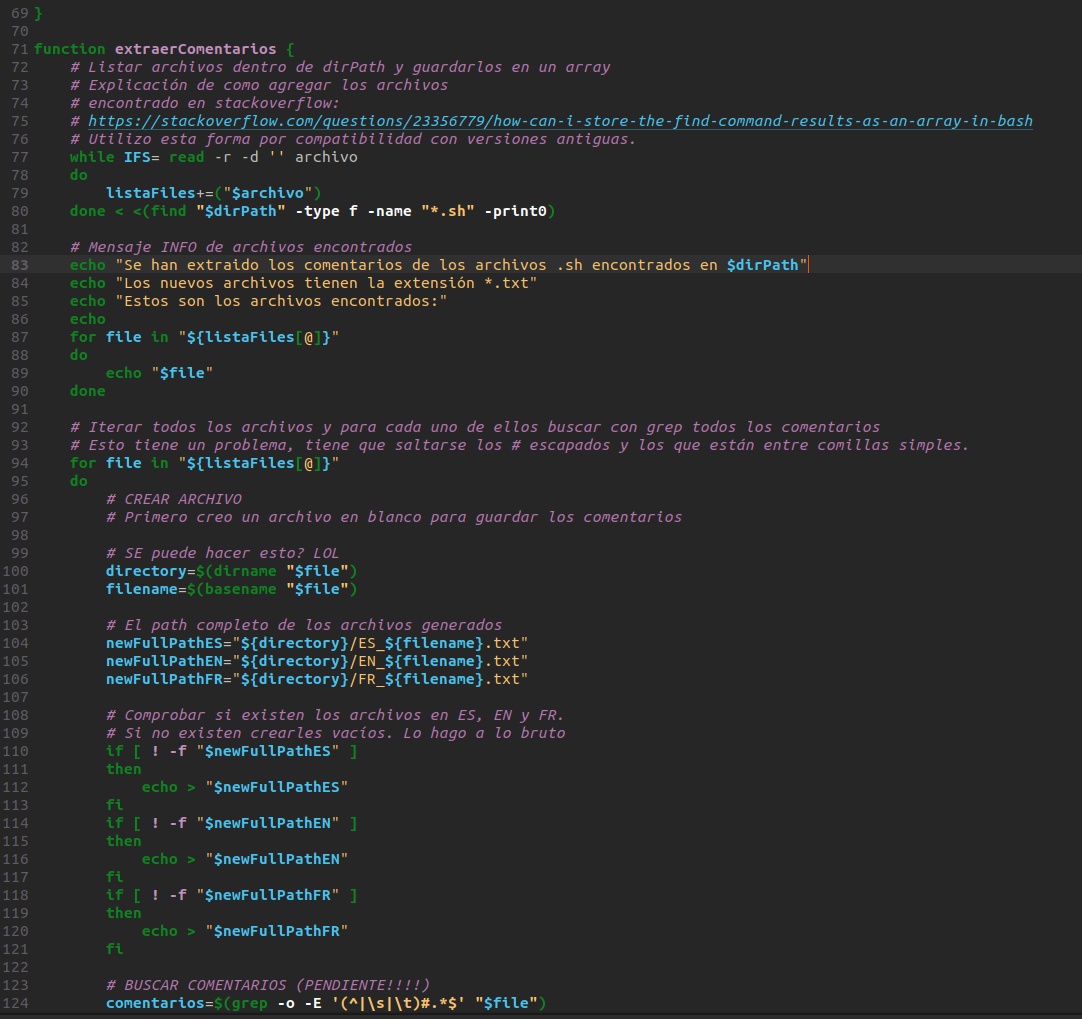
\includegraphics[width=.75\linewidth]{_1version.png}
            \caption{1ª versión del script}
        \end{figure}

    \subsection{Reinicio del proyecto con git}
        Llegado este punto he decidido crear un listado de requerimientos que necesitaba resolver. Además ahora adobte la mentalidad de resolver un problema, dejar el código funcionando, aunque no estuviese completamente satisfecho. Primero debía r\textbf{esolver la mayor cantidad de problemas} posibles, y \textbf{pulirlos a posteriori}.
        
        Para facilitarme la trazabilidad decidí iniciar un proyecto con \textbf{git}. Además, esto me permitía tener un backup sencillo de los archivos \textbf{.sh} que estaba modificando. El proyecto de git tiene dos ramas, una \textbf{main} y otra \textbf{dev} en la cual realizo todos los cambios.

        Para mayor detalle se puede recurrir al historial, así como mis anotaciones en un archivo \textbf{README.md} a modo de vitacora. Aquí se puede ver un poco el progreso y en que pensaba cada día. A parte llevaba un archivo \textbf{todo} como un recordatorio de que tenía que hacer inmediatamente a continuación en cada momento.


        \begin{figure}
            \centering
            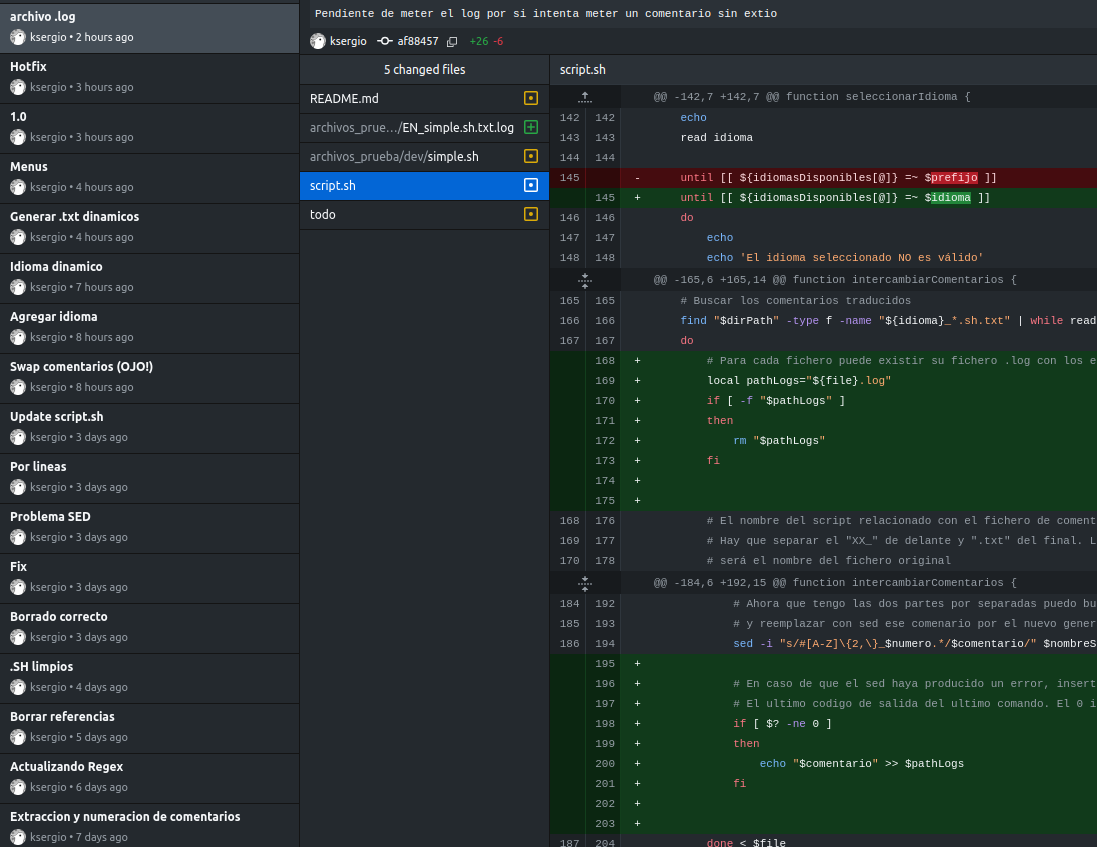
\includegraphics[width=0.75\linewidth]{_git.png}
            \caption{Historial de cambios con git}
        \end{figure}
        

\newpage
\section{Soluciones propuestas}
    \subsection{Método para buscar los comentarios con grep y find}
        Para solucionar el problema de encontrar todos los ficheros \textbf{.sh} simplemente he utilizado el comando:

        \begin{verbatim}
        find "$dirPath" -type f -name "*.sh" 
        \end{verbatim}

    Habitualmente para ser utilzado a través de un pipe con un bucle \textbf{while}. También encontré otra versión de utilizarlo que me pareció un poco menos legible

        \begin{verbatim}
        while read linea; do
            # Hacer algo con $linea
        done <<< texto.txt
        \end{verbatim}

    Para realizar la busqueda de los comentarios estoy usando un simple \textbf{grep} con una expresión regular curiosa que me he encontrado.

    Esta expresión busca el incio o el caracter \textbf{\#} separado por un espacio o tabuliación. Lo he encontrado bastante efectivo.

        \begin{verbatim}
        grep -o -E -n '(^|\s|\t)#[^!#].*$' "$file" 
        \end{verbatim}

    La opcion \textbf{E} me da acceso a las expresiones extendidas, \textbf{n} me permite insertar la linea donde se encuentra y \textbf{o} para sacar solo la parte que coincide, no toda la linea.

    \begin{verbatim}
        while IFS=: read -r numero_linea comentario
    \end{verbatim}

    Combinando con el separador \textbf{IFS=:} tenemos disponibles dos variables, el numero de linea y comentario en el bucle while.
            
    \subsection{Creación de un menú interactivo}
        Para crear el menú he copiado descaradamente los menús utilizados en la práctica de control, con una corección.

        \begin{figure}
            \centering
            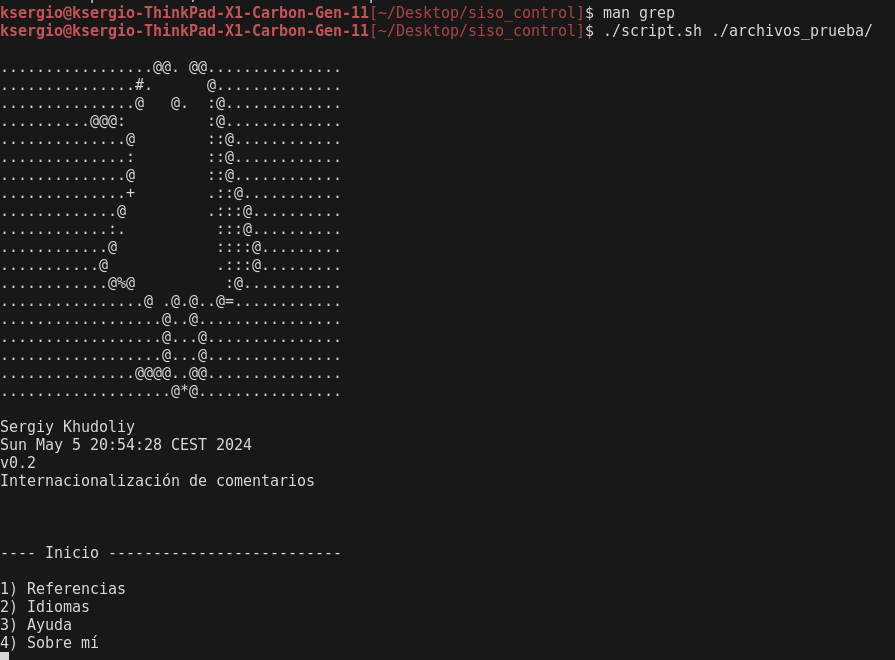
\includegraphics[width=0.75\linewidth]{_menu.png}
            \caption{Menu interactivo para seleccionar la operación}
        \end{figure}

        \newpage

        \begin{verbatim}
            function menuIdiomas {
                local opcion=0
            
                #validacion
                until ([[ $opcion > 0 && $opcion < 3 ]])
                do
                    echo
                    echo '---- Idiomas -------------------------'
                    echo
                    echo '1) Agregar'
                    echo '2) Ver disponibles'
                    echo
            
                    read opcion
                done 
            
                case "$opcion" in 
                    '1') agregarIdioma;;
                    '2') verIdiomasDisponibles;;
                esac
            }
        \end{verbatim}

        En este caso no veo la necesidad de repetir le impresión o pedir la entrada al usuario antes de realizar el bucle. Se puede hacer dentro del bucle como en el ejemplo anterior. De esta forma reduzco duplicación de código.
    
    \subsection{Borrado de comentarios en el fichero original}
        Para borrar las referencias existentes en el archivo original, lo hago usando \textbf{sed} y usando un patrón con expreisones regulares.

        \begin{verbatim}
            sed -i -e 's/#\([A-Z]\{1,\}_[0-9]*\)*/#/g' $file
        \end{verbatim}

        El formato de comentario una vez generada la referencia es del tipo \textbf{\#XX\_9999}. Dos letras y cualquier cantidad de numeros separados por un guión bajo. Este tiene un tema un poco curioso, y es que durante el desarollo tuve un error en el cual podía crear varias referencisa encadenadas. Por ejemplo; ES\_10ES\_20\_ES\_30. Con el patrón que he marcado aquí atrapo el formato todas las veces que se repita.

        En la práctia si el referenciado esta bien hecho, no debería ocurrir nunca, ya que me he tomado la molestia de borrar las referencias siempre antes de generarlas.
    
    \subsection{Creando ficheros .txt para almacenar datos}
        Una vez encontrado el \textbf{path} del fichero con el que se trabaje puedo generar los archivos necesarios para todos los idiomas. De la siguiente forma extraigo el nombre del archivo del path completo:

        \begin{verbatim}
        directorioPadre=$(dirname "$file")
        nombreFichero=$(basename "$file")
        \end{verbatim}

        Una vez que tengo el nombre del archivo ya puedo generar el nuevo fichero con el \textbf{prefijo} especifico del idioma deseado y \textbf{.txt}.
        
    \subsection{Intercambiando comentarios}
        Para intercambiar los comentarios lo que hago es buscar, de nuevo, con expresiones regulares el prefijo y el comentario.

        \begin{figure}
            \centering
            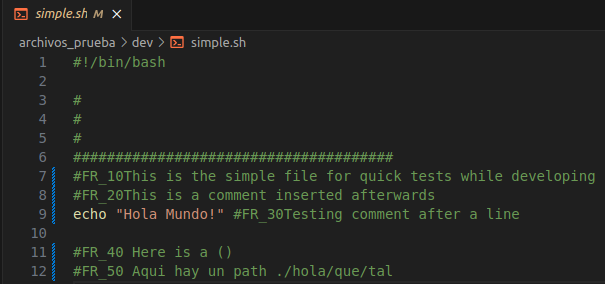
\includegraphics[width=0.75\linewidth]{_insert.png}
            \caption{Insertando comentarios de traducción}
        \end{figure}
        
        \begin{verbatim}
        's/\(.*\/\)[A-Z]\{2\}_\(.*\)\.txt$/\1\2/')
        \end{verbatim}

        Del prefijo extraigo el numero del comentario y el comentario en si, y a posteriori busco en el archivo donde se tiene que sustituir con la misma numeración.

        \begin{verbatim}
        "s/#[A-Z]\{2,\}_$numero.*/$comentario/"
        \end{verbatim}

        Un problema que me dió bastantes problemas, fue el hecho de escapar caracteres en el código. En las páginas de pruebas online donde he realizado las pruebas \textbf{regex101.com} no lo necesita, pero mi script si que se debe.
    
    \subsection{Agregando idiomas nuevos y persistencia}
        Para trabajar con distintos idiomas estoy usando un archivo oculto \textbf{.idioma} donde almaceno los idiomas como 2 letras en mayúsculas. Este archivo lo utilizo para poder persistir los datos entre ejecuciones.


        Al inicio del código siempre compruebo si existe, en caso contrario creo un archivo por defecto
        \begin{verbatim}
        function crearIdiomasStorage {
            local file='./.idiomas'
        
            # En caso de no existir crearlo de nuevo
            if [ ! -f './.idiomas' ]
            then
                touch .idiomas
                # Idiomas por defecto
                echo 'ES' >> './.idiomas'
                echo 'EN' >> './.idiomas'
            fi
        }
        \end{verbatim}

        A continuación lo carga en una array con esto. Esto es un truco curioso, pero no siempre es válido. Existen otras formas de cargar datos en un array más robustos, incluso una nueva forma para \textbf{bash >4.4} usando \textbf{readarray}.

        Yo he decidido usar una forma \textbf{curiosa} por que sí.
        \begin{verbatim}
        fileItemString=$(cat  './.idiomas' |tr "\n" " ")
        idiomasDisponibles=($fileItemString)
        \end{verbatim}

        Por otro lado previo a cualquier ejecución de alguno de las funcionalidades, siempre leo este array y solicito al usaurio que me diga con que idioma quiere trabajar. Para ello uso una variable global.
    
    \subsection{Agregando ficheros .log para errores de insertado}
        Esta es la última funcionalidad que he agregado, y no está del todo pulida. Esto queda pendiente de ser extendido, pero por ahora es la forma más básica de atajar el problema de los insertados incorrectos.


        \begin{figure}
            \centering
            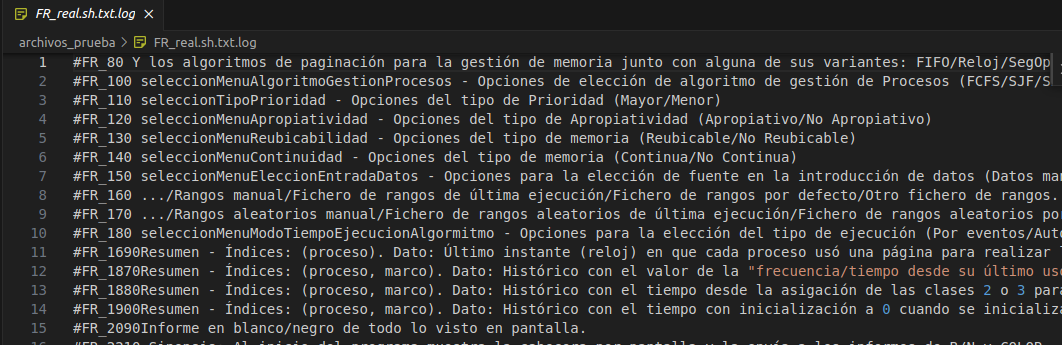
\includegraphics[width=0.75\linewidth]{_log.png}
            \caption{Archivo de log de errores al insertar comentarios}
        \end{figure}
    
        \begin{verbatim}
            if [ $? -ne 0 ]
            then
                echo "$comentario" >> $pathLogs
            fi
        \end{verbatim}

        Con este código compruebo que la ultima ejecución del comando es correcto. Lo uso después de un sed. En caso de dar un error en el insertado sale con un error 1 o 2 que será atrapado en el código.

\section{Posibles mejoras}
    \subsection{Patron regex para atrapar comentarios}
        Respecto a este apartado por ahora he encontrado que es bastante efectivo, pero puede ser que haya algunas lineas de comentario que no atrape. He creado un fichero con \textbf{corner cases} o \textbf{casos extremos}. Por ejemplo, falla para lineas que hagan echo con comillas simples que tengan un caracter \# dentro. Esto \textbf{NO} tiene por que ser un comentario.
    
    \subsection{Escapado de caracteres con sed}
        Ahora mismo para el reinsertado de comentarios de un idioma estoy usando un \textbf{sed} pero no he encontrado una forma fácil de escapar los posibles caracteres que existan en las variables usadas. Por ello, hay errores con algúnos de los insertados que están pendientes de corregir.

    \begin{figure}
        \centering
        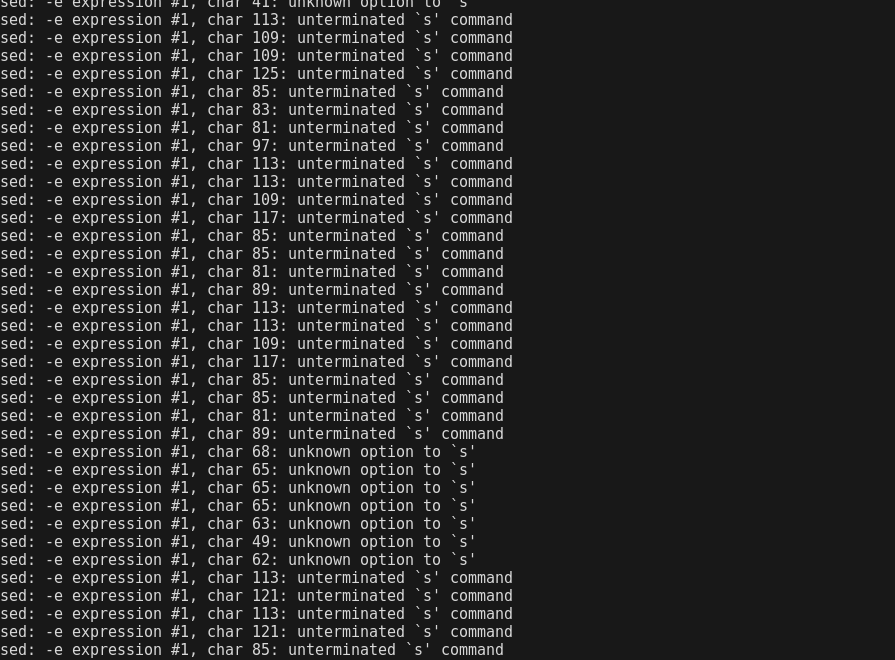
\includegraphics[width=0.75\linewidth]{_errsed.png}
        \caption{Errores en la inserción con sed}
    \end{figure}

    
    \subsection{Abuso del sed}
        Me ha resultado la forma más fácil de realizar sustituciónes en archivos. También he encontrado la sustitución de parámetros de bash, pero para ello necesito tener las dos cadenas que quiero sustituir localizadas. Para escribir en un archivo en algún lugar concreto la única forma que conozco simple era con un \textbf{sed}. Pero esto me lleva a leer el mismo entero archivo multiples veces para sustituir una única línea.

        De la misma forma para realizar saltos de linea hago llamadas multiples de \textbf{echo}, aunque entiendo que esto no es tan intensivo como la lectura de un archivo completo. En mi caso yo directamente he despreciado posibles penalizaciones por llamarlo multiples veces en vez de hacer un comentario multilinea.
    
    \subsection{Insertado de lineas problemáticas en fichero .log}
        Actualmente el insertado solo se hace si da error el sed. Pero esto no ocurre si la sustitución es vacía o no se realiza porque no se encuentra. 

        Habría que comprobar si se ha hecho al menos una inserción. Mi idea primera era revisar el archivo antes y después de cada insertado y comprobar si este ha sido modificado con un \textbf{diff} por ejemplo. Pero me resulta excesivo hacer una lectura de dos archivos para cada linea.

        Esto queda pendiente de encontrar alguna forma eficiente de comprobarse.

\newpage
\section{Conclusión personal}
    Este trabajo me ha resultado muy útil para conocer más en profundidad los comandos disponibles de \textbf{Linux}, sus opciones y peculiaridades.

    Siempre he deseado aprender el lenguaje \textbf{bash} pero nunca he tenido disponibilidad y he utilizado sustitutos para el scripting como \textbf{Python}. Por un lado me parece más legible y obviamente más flexible y potente, pero por otro lado esto supone agregar \textbf{complejidad adicional} y alejarme de las herramientas que ya provee el propio \textbf{sistema operativo}.

    Además usar otro lenguaje implica posibles puntos de fallo adicional, en cambio con bash estamos trabajando directamente con el sistema. No conozco si existe una diferencia de rendimiento importante utilizando estos dos lenguajes, pero entiendo que este debe ser más eficiente.

    En definitiva, me alegra el haber tenido la oportunidad de realizar un trabajo para ampliar mi repertorio y forma de pensar.

\end{document}
